\section{Die Eulersche Zahl auf 1.000.000 Stellen}
Bevor ich die Eulersche Zahl auf eine Million stellen berechnen wollte, hatte ich sie mithilfe eines Python-moduls für arbiträre Präzision bereits auf einhunderttausend Stellen berechnet. Durch einen Verwandten dann über den sog. Tröpfelalgorithmus hingewiesen, mit dem man die Eulersche Zahl von allein in arbiträrer Präzision berechnen kann.
\subsection{Der Tröpfelalgorithmus}
Der Tröpfelalgorithmus funktioniert folgendermaßen:
\begin{table}[h]
\centering
\begin{tabular}{|l|llllll|}
\hline
\rowcolor[HTML]{CBCEFB} 
  & 2 & 3 & 4 & 5 & 6 & 7 \\ \hline
2 & 1 & 1 & 1 & 1 & 1 & 1 \\
\rowcolor[HTML]{DAE8FC} 
7 & 0 & 1 & 0 & 1 & 5 & 3 \\
1 & 1 & 1 & 3 & 4 & 0 & 1 \\
\rowcolor[HTML]{DAE8FC} 
8 & 0 & 1 & 2 & 0 & 2 & 6 \\ \hline
\end{tabular}
\caption{Kleine Tabelle zur Veranschaulichung / als Beispiel}
\end{table}
\par Erstelle eine Tabelle. Reihe 0 besteht aus einer leeren Stelle am Anfang und danach 2,3,4,... bis zu einer Zahl n, sodass n! die so viele Stellen hat wie man Nachkommastellen berechnen möchte. Reihe 1 beginnt mit einer 2 (welches bereits die Vorkommastelle von $e$ darstellt) und ist von nur Einsen gefolgt. Um die nächste Reihe zu berechnen, beginne ganz rechts in der jetzigen Spalte und multipliziere das Feld mit 10, teile das durch das Feld darüber in Zeile 0, schreibe den Rest in das untere Feld und addiere den Übertrag zum Feld rechts, nachdem man den Wert dort ebenfalls mal 10 multipliziert hat (im Fall man ist ganz links angekommen, dann schreibt man den Übertrag unten rechts in die Reihe der Nachkommastellen). Wenn man diesen Vorgang wiederholt, dann erscheinen die Ziffern von $e$ in basis 10 als die erste Reihe der Tabelle.
\subsubsection{Die Genauigkeit des Tröpfelalgorithmus}
Anders als die anderen Näherungen, die ich mir angesehen habe, müsste der Tröpfelalgorithmus schneller als linear wachsen. für eine Spalten-Anzahl von x gibt es ungefähr $\log_{10}{(x!)}$ Nachkommastellen
\begin{figure}[h]
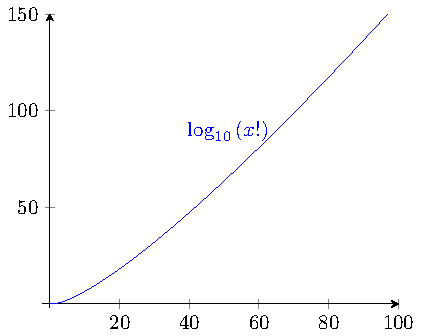
\includegraphics{medien2/log10/log.pdf}
\centering
\caption{Genauigkeit des Tröpfelalgorithmus'}
\end{figure}
\par Für kleine Werte von x sieht der Graph linear aus und verdächtig ähnlich zu Abbildung 2: dem Graphen über die Summation. Und tatsächlich basiert der Tröpfelalgorithmus von der Idee her auf der Näherung der Summation. \[
  \sum_{n=0}^\infty{ \frac{n!}{n^n} } = 1 + 1 + \frac{1}{2} + \frac{1}{6} +\frac{1}{24} + \dots = 2 + \frac{1}{2}(1+ \frac{1}{3}(1+\frac{1}{4}(\dots)))
\] $e$ ist in der fakultätsbasierte Base periodisch ($2,\overline1$) und das wird ausgenutzt um die Reihe 0 zu bilden.
\subsection{1.000.000 stellen und abschließende Worte}
\par Die Eulersche Zahl beginnt mit den Ziffern 2.71828182845\dots, und die Ziffern bis 1.000.000 sind \dots98176447694228188\dots{} (die Datei ist als Anhang digital mit in der Arbeit enthalten) und dann geht es noch lange weiter. Das Arbeiten an dem Thema hat mir sehr gefallen und ich habe einiges dazu gelernt. Wenn Ich die Arbeit nocheinmal von vorn schreiben könnte, dann würde ich mich mehr auf die Organisation konzentrieren und noch gründlicher arbeiten.
